\documentclass[11pt]{article}

\usepackage[margin=1in]{geometry}
\usepackage{amsmath,amssymb}
\usepackage{booktabs}
\usepackage{graphicx}
\usepackage{array}
\usepackage{tabularx}
\usepackage{caption}
\usepackage{xcolor}
\usepackage[hidelinks]{hyperref}
\usepackage{microtype}
\usepackage{fontspec}
\usepackage{newtxmath}
\usepackage{titlesec}
\usepackage{titling}

\newcommand{\note}[1]{\texorpdfstring{\textcolor{red}{[NOTE: #1]}}{[NOTE: #1]}}
\newcolumntype{Y}{>{\raggedright\arraybackslash}X}
\defaultfontfeatures{Ligatures=TeX}
\setmainfont{IBM Plex Serif}[
  Path=../../../addenda/typst-field-manual/assets/fonts/,
  UprightFont=IBMPlexSerif-Regular.ttf,
  BoldFont=IBMPlexSerif-Bold.ttf,
  ItalicFont=IBMPlexSerif-Italic.ttf,
]
\setsansfont{IBM Plex Sans Condensed}[
  Path=../../../addenda/typst-field-manual/assets/fonts/,
  UprightFont=IBMPlexSansCondensed-Regular.ttf,
  BoldFont=IBMPlexSansCondensed-Bold.ttf,
]
\setmonofont{IBM Plex Mono}[
  Path=../../../addenda/typst-field-manual/assets/fonts/,
  UprightFont=IBMPlexMono-Regular.ttf,
]
\emergencystretch=2em
\definecolor{specteraccent}{HTML}{1F4555}
\definecolor{spectermuted}{HTML}{616161}

\setlength{\droptitle}{-2.0em}
\pretitle{%
  \begin{flushleft}%
  \color{specteraccent}\rule{\linewidth}{1.2pt}\par
  \vspace{0.85em}%
  {\sffamily\bfseries\small SPECTER LABS PREPRINT\par}%
  \vspace{0.8em}%
  \LARGE\bfseries
}
\posttitle{\par\end{flushleft}\vspace{0.45em}}
\preauthor{\begin{flushleft}\normalsize\sffamily}
\postauthor{\par\end{flushleft}\vspace{0.25em}}
\predate{\begin{flushleft}\small\sffamily\color{spectermuted}}
\postdate{\par\end{flushleft}\vspace{0.95em}}

\titleformat{\section}
  {\normalfont\large\sffamily\bfseries\color{specteraccent}}
  {\thesection.}{0.6em}{}
\titleformat{\subsection}
  {\normalfont\normalsize\sffamily\bfseries}
  {\thesubsection.}{0.6em}{}
\titlespacing*{\section}{0pt}{1.8ex plus .2ex minus .2ex}{0.8ex}
\titlespacing*{\subsection}{0pt}{1.4ex plus .2ex minus .2ex}{0.55ex}
\captionsetup[figure]{font=small,labelfont=bf,textfont=it}
\captionsetup[table]{font=small,labelfont=bf}

\renewenvironment{abstract}{%
  \begin{flushleft}
  \small
  {\sffamily\bfseries Abstract\par}
  \vspace{0.35em}
}{%
  \end{flushleft}
  \vspace{0.65em}
}

\title{Sorting Cells as Morphogenesis, Revisited:\\Mechanisms, Ablations, and Robustness Semantics}
\author{%
  \begin{tabular}{@{}p{0.38\linewidth}@{\hspace{2.5em}}p{0.38\linewidth}@{}}
  Ludwig Pouey & Phil Rohr \\
  {\small\color{spectermuted}Specter Labs} & {\small\color{spectermuted}Specter Labs}
  \end{tabular}
}
\date{February 2026, revised October 2026}

\begin{document}
\maketitle

\begin{abstract}
Zhang et al.\ (2024) propose a minimal morphogenesis model in which individual ``cells'' execute
classical sorting rules from a local cell-view state and nonetheless achieve global organization.
In these implementations the operator class is not uniform, since Bubble, Insertion, Gnome, and
Shaker use adjacent swaps whereas 1D Selection performs direct transpositions toward an ideal
position. We revisit the model by separating action range, blocked-target policy, and execution
substrate, and by scoring algotype clustering against a label-permutation null computed on each
run's own trajectory.

Scored against that null, algotype clustering appears only in mixtures where one class moves late.
Pairs that contain Insertion, whose sorted-prefix gate delays its cells, cluster above the null,
and removing the gate (\texttt{InsertionNoWait}) returns clustering to the null, where the ungated
Bubble, Gnome and Shaker mixtures also sit. Transplanting the same gate onto Bubble and Gnome
clones raises both temporal separation and clustering to the level of native Insertion while the
ungated clones stay at the null, which gives the efficiency hypothesis of Zhang et al.\ a first
causal test. Selection mixtures without Insertion cluster weakly without temporal separation, so
timing does not account for all of the clustering in the original set.

The robustness experiments mostly confirm consequences of the rule definitions. Under immovable
frozen indices only long-range Selection with frozen-target rerouting can complete, because
adjacent moves cannot carry values across a frozen index and a stubborn cell waits forever on one;
cell-view and centralized implementations that share the skip-frozen rule agree in every paired
trial; and threaded and sequential schedules of the same cells agree in outcome and do the same
work (ratios $0.97\times$ to $1.02\times$) once frozen cells, as in the original code, run no
thread. We report $K_{\mathrm{state}}$, an exact reachable-state proposal null, and find it set
mostly by the size of the reachable state space, $1.7$ to $2.6$ units below
$\log_{10}(n_{\text{active}}!)$ for every algorithm that finishes, and we keep the 2D and Directed
Flow results as narrower diagnostics.

\end{abstract}

\section{Introduction}
\label{sec:intro}
Local-to-global organization is a recurring motif in both developmental biology and distributed
computing. Zhang et al.\ introduce a toy model that intentionally collapses the substrate to its
barest computational ingredients: a 1D line (or 2D grid) of agents that update from a local
cell-view state according to simple rules derived from classical sorting algorithms
\cite{zhang2024classical}. Many of those rules use adjacent swaps, but the published 1D Selection
implementation instead performs direct transpositions toward an explicit ideal position.
Despite minimal sensing and communication, the system exhibits:
(i) reliable convergence to an ordered configuration in 1D,
(ii) algotype clustering (cells running the same algorithm become spatially adjacent),
and (iii) robustness to perturbations such as frozen (damaged) cells.

This follow-up has a deliberately narrow scope: we do not propose a new model class.
Instead, we push the original claims by adding targeted measurements and ablations, and by clarifying
semantics that strongly affect conclusions.

\paragraph{Guiding questions.}
We focus on seven questions:
\begin{enumerate}
  \item \textbf{Mechanism:} what is the minimal causal mechanism sufficient to explain algotype
  clustering?
  \item \textbf{Operator classes:} which parts of Selection's robustness come from action range,
  and which come from frozen-target rerouting?
  \item \textbf{Ablation:} within the published Selection operator class, which specific rule is
  responsible for robustness and ``navigation'' in the presence of obstacles?
  \item \textbf{Robustness comparison:} does the cell-view advantage over traditional algorithms
  survive when both handle frozen indices the same way, and does the threaded execution substrate
  add anything to it?
  \item \textbf{Dimensionality:} which behaviors generalize to 2D ordering targets, and what fails?
  \item \textbf{Structure in dynamics:} do swap-interaction graphs expose algorithmic signatures that
  align with (or fail to predict) task success?
  \item \textbf{Search efficiency:} can we quantify how much ``smarter'' each algorithm is relative to
  a blind random-walk baseline, using the K-computation framework of Chis-Ciure and Levin
  \cite{chisciure2025cognition}?
\end{enumerate}

\paragraph{Summary of findings.}
Clustering excess over the label-permutation null tracks temporal separation in mixtures with a
waiting gate, and the gate ablation and the gate transplant both move clustering in the direction
the timing account predicts, with ungated mixtures sitting at the null. Selection mixtures cluster
weakly without separation, which leaves part of the original clustering unexplained. Under
immovable obstacles the factorization, rerouting ablation, centralized comparison and
matched-substrate comparison all come out the way the rule definitions require, so we present them
as consistency checks on the implementation: only long-range rerouting Selection can reach the
sorted state, matched baselines reproduce the same paired outcomes, and threaded and sequential
schedules do the same work. The 2D section and Directed Flow remain secondary, and the K section
is presented as $K_{\mathrm{state}}$, a scalable exact state-proposal surrogate for the
intractable full operator-walk K at $n=30$.

\section{Model and Metrics}
\label{sec:methods}
\subsection{Sorting cells and operator classes}
We adopt the Zhang et al.\ multithreaded ``cell-view'' implementation: each cell is a thread that
repeatedly decides whether to swap using only bounded local state and shared state protected by a
lock. ``Cell-view'' therefore describes the decision substrate, not a uniform move operator.
Cells are parameterized by an \emph{algotype} (Bubble, Selection, Insertion, etc.), and those
algotypes differ materially in target representation and action range.

\begin{table}[t]
  \centering
  \small
  \begin{tabularx}{\linewidth}{@{}Y Y Y Y@{}}
    \toprule
    Algorithm family & Target representation & Executed move & Blocked-target behavior \\
    \midrule
    Bubble / Insertion / Gnome / Shaker (1D) & Local neighbor comparisons; Insertion also tracks a sorted-prefix gate & Adjacent swap & No rerouting beyond the local rule \\
    Selection (published 1D) & Explicit ideal index in the 1D total order & Direct transposition to the ideal index & Reroute when the desired target index is frozen, or remain stubborn in the ablation \\
    Adjacent Selection & Same explicit ideal index as 1D Selection & One adjacent step toward the ideal index & Same rerouting / stubborn split as above \\
    Selection2D & Explicit ideal position induced by the target order & Neighbor-local greedy grid swap & No long-range transposition; progress is routed through adjacent moves \\
    \bottomrule
  \end{tabularx}
  \caption{Operator classes discussed in this paper. The key distinction is between local
  perception and action range: published 1D Selection has local cell-view execution but a nonlocal
  move operator.}
  \label{tab:operator-classes}
\end{table}

\subsection{Obstacle semantics}
The original paper discusses both movable and immovable damage. In the published code, the term
``frozen cell'' is therefore overloaded; two distinct semantics matter:
\begin{itemize}
  \item \textbf{Movable frozen cells:} frozen cells do not initiate swaps, but can be displaced by
  other cells swapping with them (a ``movable obstacle'').
  \item \textbf{Immovable frozen indices:} certain array indices cannot participate in swaps at all
  (an ``immovable obstacle'' / hard barrier).
\end{itemize}
We use the terms \emph{movable} and \emph{immovable} throughout; each result section states the
semantics explicitly. A compact per-experiment semantics summary and command index are collected in
Appendix~\ref{sec:appendix-repro} so the main text can stay focused on the argument.

\subsection{Clustering}
For a 1D array of length $n$ with algotypes assigned to positions, define instantaneous clustering
$C(t)$ as the fraction of adjacent pairs that share the same algotype, recorded after every swap.
Let $p_t$ be the fraction of cells of type $t$. Earlier versions of this paper reported
$\Delta C = \max_t C(t) - \sum_t p_t^2$, but the maximum of a noisy curve over several hundred
states sits well above $\sum_t p_t^2$ even when both halves of the array run the same rule (about
$0.14$ above it at $n=50$), and the exact random-mixing expectation for adjacent matches at a
$25/25$ split is $24/49$ rather than $0.5$. We therefore score each run against a label-permutation
null on its own trajectory: the algotype labels are shuffled across cell values $200$ times,
$\max_t C(t)$ is recomputed for each shuffle on the same sequence of value arrangements, and the
reported \emph{clustering excess} is
\[
E \;=\; \max_t C(t) \;-\; \mathbb{E}_{\pi}\!\left[\max_t C_{\pi}(t)\right].
\]
The null holds trajectory length and sorting dynamics fixed and asks only whether the cells that
become adjacent depend on their type. The result files also carry the same excess for the
time-averaged $C(t)$, a per-trial permutation $p$-value, and the raw $\Delta C$ for comparison with
the original figures.

\subsection{Temporal separation}
We define an algorithm's \emph{normalized mean move time} as the average time index (normalized to
$[0,1]$ over the swap sequence) at which cells of that type participate in swaps. For a pair
$(a,b)$, temporal separation is:
\[
S(a,b) \;=\; \left|\mu_a - \mu_b\right|.
\]

\subsection{Dips (``delayed gratification'')}
We operationalize a ``dip'' as a transient increase in a global error metric (1D monotonicity errors
or 2D inversion count) that subsequently recovers to at most the starting value. We use the same dip
detection logic across 1D and 2D trajectories.

\section{Results}
\label{sec:results}

\subsection{Temporal separation and clustering}
Figure~\ref{fig:temporal-clustering} plots clustering excess against temporal separation for the
ten pairwise mixtures of five algotypes (Bubble, Selection, Insertion, Gnome, Shaker; $n=30$, $50$
trials per pair). The four Insertion pairs have the largest separations ($0.12$ to $0.21$) and all
cluster above the null ($E$ between $+0.051$ and $+0.090$), while the three pairs of ungated
adjacent-swap rules (Bubble, Gnome, Shaker) sit at the null. The three Selection pairs without
Insertion cluster weakly ($+0.026$ to $+0.031$) at separations of $0.04$ to $0.05$, so the
correlation across all ten pairs ($r = 0.94$) is carried by the Insertion family and falls to
$r = 0.43$ across the six pairs without Insertion. Temporal separation accounts for the clustering
in gated mixtures, and Selection mixtures cluster by some other route that we have not identified.
One candidate is that Selection's long-range transpositions carry runs of same-type cells into the
sorted prefix together, which a chimera of Bubble with an adjacent-only Selection variant would
test.

The timing account goes back to Zhang et al., who proposed as an efficiency hypothesis that
efficient algotypes move first and slower ones catch up. Insertion cells activate late because
their sorted-prefix gate delays participation until the left portion of the array is already
ordered, so the late swap bursts involve mostly one class, and cells that move during the same
burst are more likely to end up adjacent because they are the only cells still rearranging. The
effect resembles heterochrony in developmental biology, where shifts in the relative timing of
developmental processes generate spatial structure without type-recognition signals.

\begin{figure}[t]
  \centering
  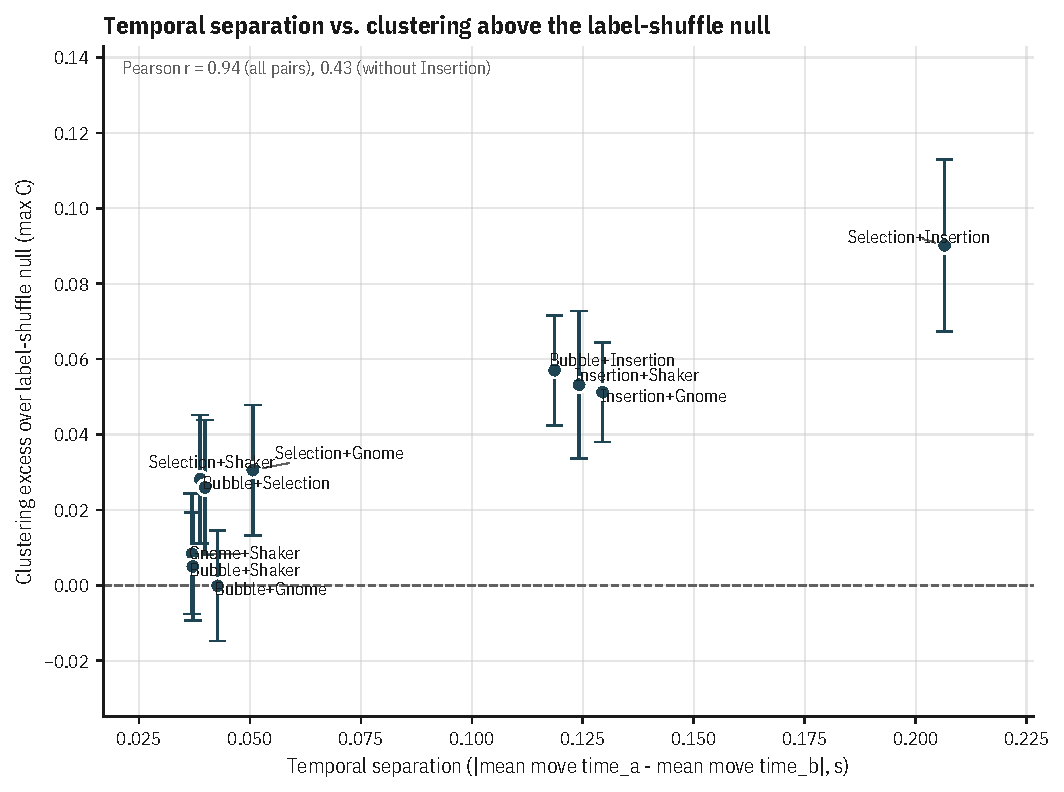
\includegraphics[width=0.85\linewidth]{figures/fig1_temporal_vs_clustering.pdf}
  \caption{\textbf{Temporal separation and clustering excess.}
  Each point is an algorithm pair; $x$ is temporal separation computed from per-algotype normalized
  mean move times, and $y$ is the clustering excess $E$ over the label-permutation null (dashed
  line at zero). Error bars show 95\% confidence intervals
  ($\text{mean} \pm 1.96 \cdot \sigma / \sqrt{n}$, $n=50$ trials per pair, $30$ cells).}
  \label{fig:temporal-clustering}
\end{figure}

\subsection{Ablation: removing Insertion's waiting gate returns clustering to the null}
If temporal separation causes the clustering in Insertion mixtures, removing the gate that makes
Insertion late should remove it. We implement \texttt{InsertionNoWait} by deleting the
enable-to-move check, so that Insertion cells move from the start like the other local rules. Over
$20$ trials with $50$ cells, Bubble+Insertion clusters above the null ($E = +0.079$, 95\% CI
$+0.054$ to $+0.105$), while Bubble+InsertionNoWait returns to the null ($E = -0.007$, CI $-0.020$
to $+0.007$) beside the ungated control Bubble+Gnome ($E = +0.011$, CI $-0.004$ to $+0.026$), as
Figure~\ref{fig:clustering-ablation} shows. An earlier version of this figure sampled $C(t)$ every
$0.02$\,s of wall-clock time, which gave the slower gated condition more samples and therefore a
higher maximum, and reported raw $\Delta C$ values of $0.166$, $0.091$ and $0.073$. With $C(t)$
recorded after every swap the raw values are $0.190$, $0.131$ and $0.149$, and the two ungated
conditions sit exactly where their own label-shuffled trajectories put them.

\begin{figure}[t]
  \centering
  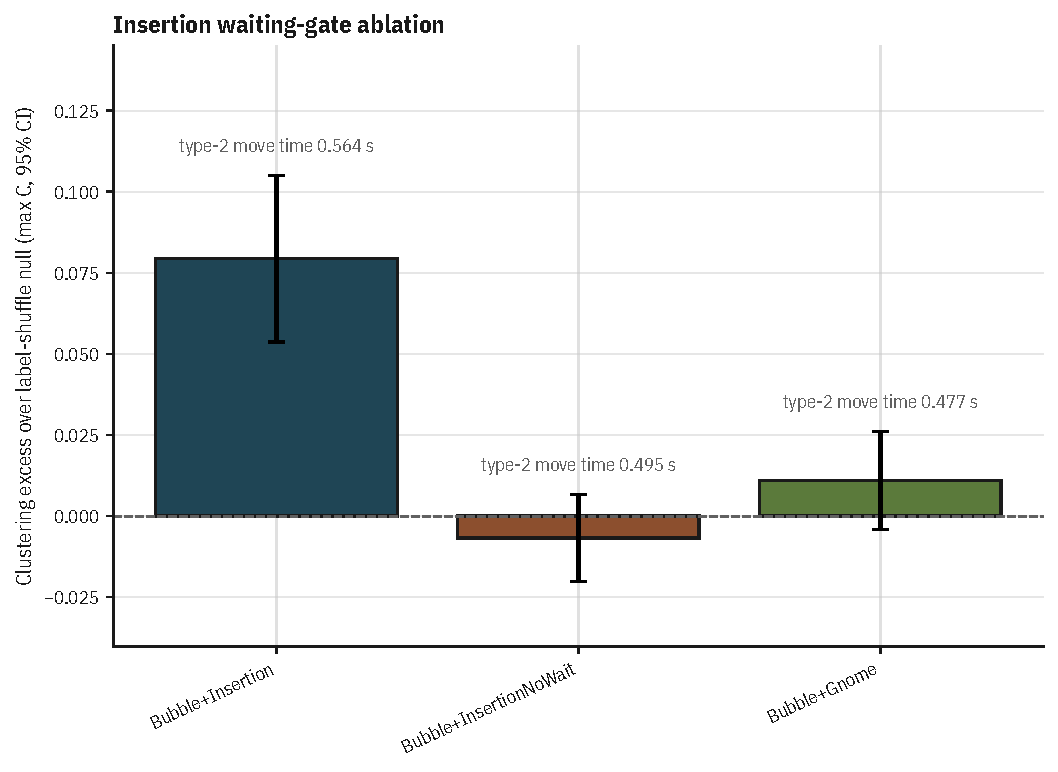
\includegraphics[width=0.85\linewidth]{figures/fig2_clustering_ablation.pdf}
  \caption{\textbf{Insertion waiting-gate ablation.}
  Clustering excess $E$ over the label-permutation null (dashed line at zero) with 95\% confidence
  intervals, over $20$ trials with $50$ cells and $C(t)$ recorded after every swap.
  Bubble+Insertion clusters above the null, while Bubble+InsertionNoWait and the ungated control
  Bubble+Gnome sit at it. Annotations give the mean move time of the second algotype.}
  \label{fig:clustering-ablation}
\end{figure}

\subsection{Synthetic waiting gates transfer clustering beyond Insertion}
If the gate carries the effect, exporting the same sorted-prefix wait to another local rule should
raise both temporal separation and clustering while the swap rule stays fixed. We pair each base
algorithm with a labelled clone that has no gate and with a delayed clone that keeps the same swap
rule and adds the Insertion-style wait.

Across $30$ trials per pair ($3$ seeds $\times$ $10$ trials, $50$ cells), Bubble+DelayedBubble
reaches separation $0.114$ and excess $E = +0.064$ (CI $+0.050$ to $+0.078$), against $0.024$ and
$+0.017$ (CI $0.000$ to $+0.034$) for Bubble+BubbleClone, and Gnome+DelayedGnome reaches $0.107$
and $+0.052$ (CI $+0.034$ to $+0.069$), against $0.025$ and $+0.006$ (CI $-0.011$ to $+0.023$) for
Gnome+GnomeClone. Both delayed pairs land beside native Bubble+Insertion (separation $0.103$,
$E = +0.061$), while Bubble+InsertionNoWait sits at the null (separation $0.025$, $E = +0.001$).
The excess of the time-averaged $C(t)$ gives the same ordering ($+0.058$, $+0.047$ and $+0.056$ for
the three gated pairs, $+0.016$ or less for the three ungated ones). The per-trial permutation test
clears the 1-in-20 level in only $6$ of $30$ trials for each gated pair, so the transfer is a
population effect that $30$ trials resolve and single runs mostly do not.

This gives the efficiency hypothesis of Zhang et al.\ its first causal test, in which a wait
transplanted onto an otherwise unchanged rule reproduces the clustering of native Insertion while
the same rule without the wait sits at the null. The raw $\Delta C$ values ($0.173$ against $0.156$
for the Bubble family) made the transfer look marginal in the earlier version of this paper,
because $0.11$ to $0.14$ of every raw value is the peak that a label-shuffled trajectory also
reaches.

\begin{figure}[t]
  \centering
  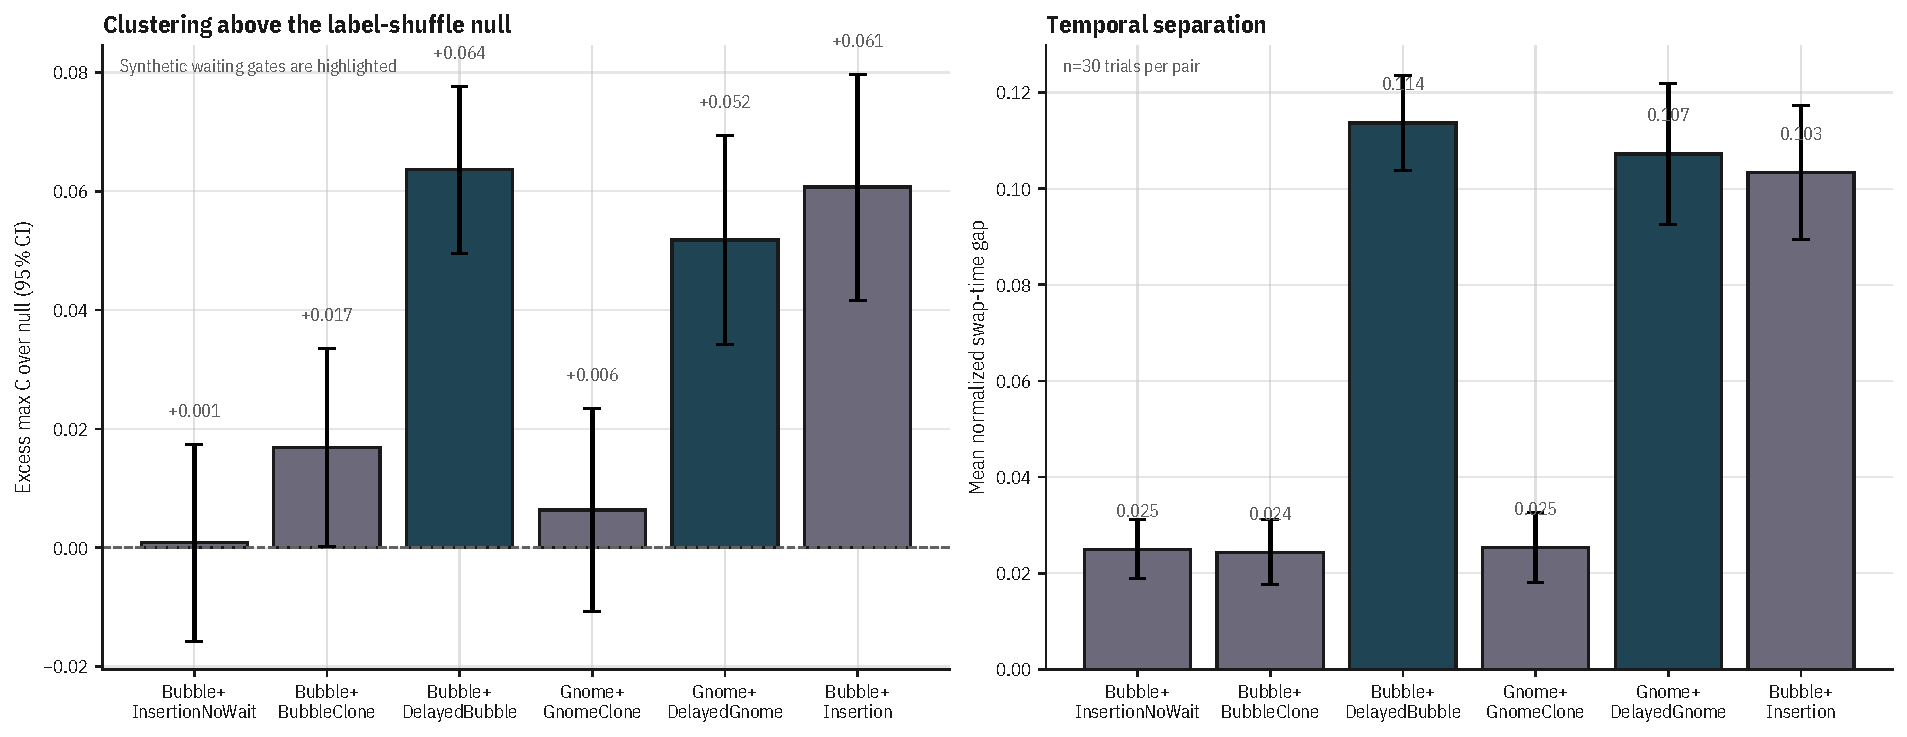
\includegraphics[width=\linewidth]{figures/fig9_timing_interventions.pdf}
  \caption{\textbf{Synthetic waiting gates transfer clustering beyond Insertion.}
  Left: clustering excess $E$ over the label-permutation null with 95\% confidence intervals.
  Right: temporal separation with 95\% confidence intervals. Same-family clones without the
  waiting gate sit at the null and in the low-separation regime, while delayed Bubble and delayed
  Gnome clones match the Bubble+Insertion reference condition.}
  \label{fig:timing-transfer}
\end{figure}

\subsection{Selection factorization under matched obstacle semantics}
The factorization experiment decomposes Selection robustness into two axes:
(i) action range (direct transposition vs.\ adjacent step) and
(ii) blocked-target behavior (rerouting vs.\ stubbornness).
All four variants share the same 1D ideal-position target representation; only the executed move and
blocked-target policy change.

The immovable panel uses $n=30$, timeout $5$s, seeds $\{40,41,42\}$, and $10$ paired trials per
condition (30 trials total). The movable control uses the same seeds with $5$ paired trials per
condition (15 trials total), tying the factorization back to the original paper's damaged-cell
semantics.

Figure~\ref{fig:exp25} and Table~\ref{tab:exp25} show that under immovable barriers only the
long-range+routing quadrant succeeds once frozen indices are introduced, and each failure follows
from the rule definitions. A long-range stubborn cell whose target index is frozen keeps pointing
at it and can never complete its swap. Adjacent active-active moves cannot exchange values across
an immovable frozen index, so for both adjacent variants every sampled trial at frozen counts
$\{3,6,9\}$ is unreachable for any adjacent policy, and these arms fail by reachability rather than
by policy. The adjacent variants stay strictly local (weighted mean swap span $1.00$) and keep
swapping inside their segments until the timeout, so at frozen$=3$ adjacent+routing averages
$14{,}077$ swaps and adjacent+stubborn $6{,}831$, against $91$ for long-range+routing. Under the
movable control ($15$ trials per condition) long-range+routing succeeds in $3/15$ trials at one
frozen cell and the other three variants in none once any frozen cell is present.

We read the factorization as a consistency check on the implementation, confirming that the
published 1D Selection behaves as a long-range rule with a frozen-target branch and should not be
treated as another local adjacent-swap rule. The rerun leaves frozen cells without threads, as the
original code does; the success counts are unchanged from the earlier archive, and the swap counts
of the failing adjacent arms are somewhat lower.

\begin{table}[t]
  \centering
  \small
  \begin{tabular}{@{}lrrrr@{}}
    \toprule
    Variant & Frozen=0 & 3 & 6 & 9 \\
    \midrule
    Long-range + rerouting & 30/30 & 30/30 & 30/30 & 30/30 \\
    Long-range + stubborn & 30/30 & 0/30 & 0/30 & 0/30 \\
    Adjacent + rerouting & 30/30 & 0/30 & 0/30 & 0/30 \\
    Adjacent + stubborn & 30/30 & 0/30 & 0/30 & 0/30 \\
    \bottomrule
  \end{tabular}
  \caption{\textbf{Selection factorization under immovable semantics.}
  Success counts across the $2\times2$ factorization of action range and blocked-target policy.
  Each condition aggregates $30$ paired trials ($3$ seeds $\times$ $10$ trials). Only the
  published long-range+routing combination can reach the sorted state once immovable frozen
  indices are introduced; the adjacent arms have no reachable trial instances there.}
  \label{tab:exp25}
\end{table}

\begin{figure}[t]
  \centering
  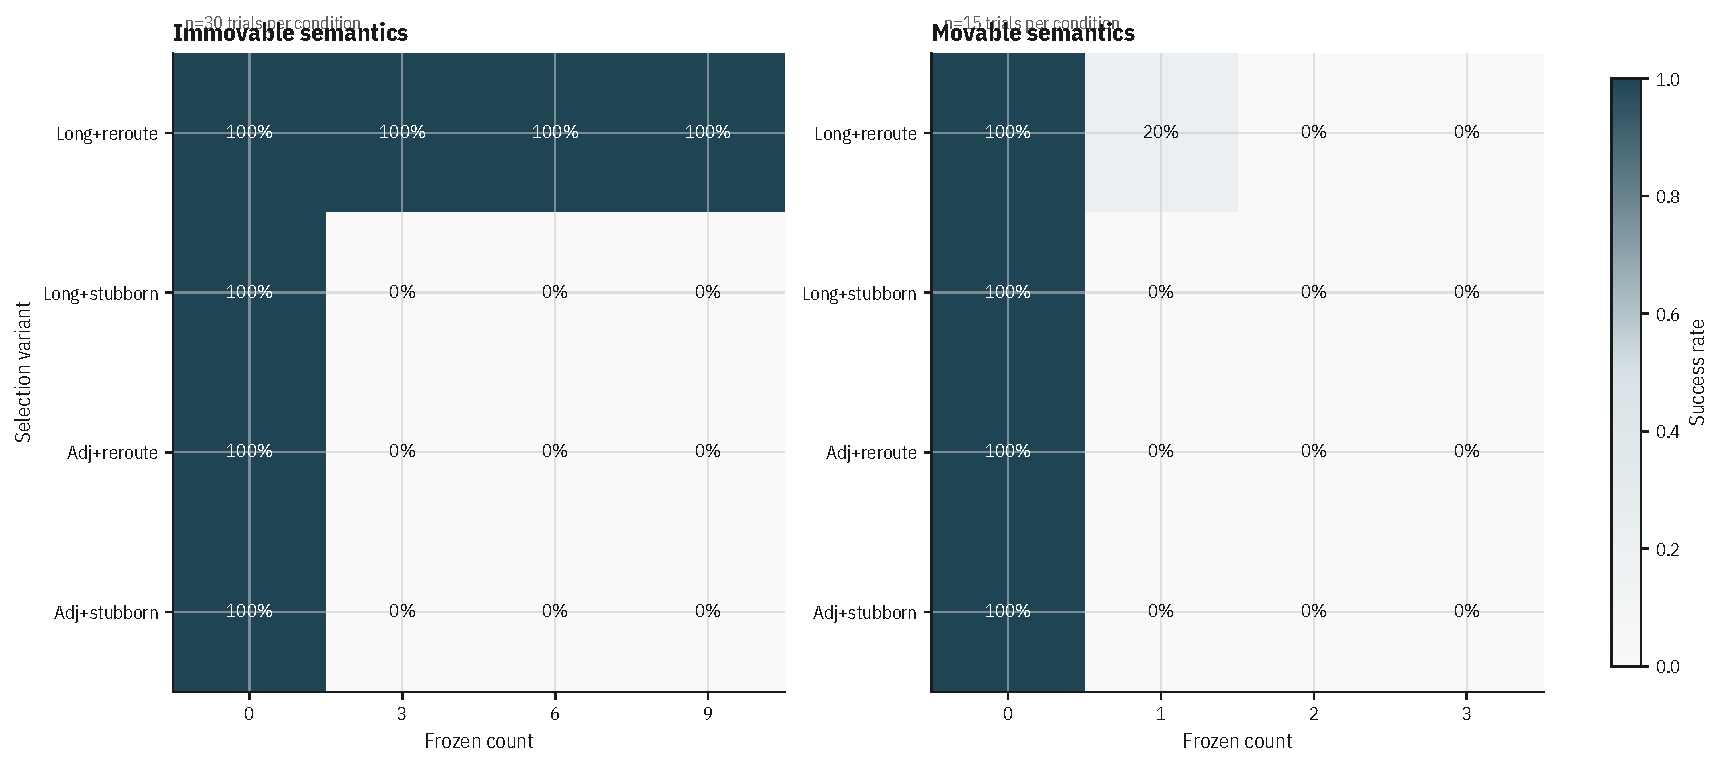
\includegraphics[width=\linewidth]{figures/fig7_selection_factorization.pdf}
  \caption{\textbf{Selection factorization across obstacle semantics.}
  Left: immovable frozen indices. Right: movable frozen cells. Under immovable barriers, only the
  published long-range+routing variant remains successful once obstacles are introduced. Under the
  original movable-damage regime ($15$ trials per condition) even that quadrant succeeds in only
  $3/15$ trials at one frozen cell, so obstacle semantics change which variants can succeed.}
  \label{fig:exp25}
\end{figure}

\subsection{Frozen-target rerouting within the published Selection operator class}
The rerouting ablation isolates the rerouting half of the factorization within the original
long-range Selection operator class. \texttt{StubbornSelectionCell} keeps the same direct-target
transposition operator and still updates its active target in some cases, but it removes the
specific reroute that occurs when the desired target index is frozen.

We ran the ablation with $n=30$ cells, $30$ trials per condition, timeout $10$s, and immovable
frozen-index semantics, aggregated across seeds $\{40,41,42\}$ (90 trials per frozen-count
condition). Across frozen counts $\{3,6,9\}$, adaptive Selection succeeds in $270/270$ trials and
the stubborn ablation in $0/270$. The result is close to definitional: under immovable semantics a
Selection cell that keeps pointing at a frozen index can never complete its swap, so the stubborn
failures follow from the rule, and the trial counts confirm that the implementation behaves as
written. These counts come from the earlier archive, which also started threads for frozen cells
and whose per-seed files were not retained (Appendix~\ref{sec:appendix-repro}).

\begin{table}[t]
  \centering
  \small
  \begin{tabular}{@{}lrr@{}}
    \toprule
    Frozen & Adaptive Selection & Stubborn Selection \\
    \midrule
    0 & 90/90 & 90/90 \\
    3 & 90/90 & 0/90 \\
    6 & 90/90 & 0/90 \\
    9 & 90/90 & 0/90 \\
    \bottomrule
  \end{tabular}
  \caption{\textbf{Frozen-target rerouting ablation, 3-seed aggregate.}
  Success counts under immovable frozen indices. Each condition aggregates $90$ trials
  ($3$ seeds $\times$ $30$ trials). Read together with the factorization result, this supports a narrower and
  stronger claim: rerouting is necessary for robustness \emph{within} the published long-range
  Selection operator class.}
  \label{tab:exp10}
\end{table}

\subsection{Cell-view vs.\ centralized robustness under matched frozen-index semantics}
The original paper compares cell-view sorting with traditional sorting under frozen cells and
reports lower final error for the cell-view versions. That comparison sets cell-view algorithms
against traditional algorithms that also differ in how they handle a frozen cell, so it leaves open
whether the gap comes from the cell-view implementation or from the frozen-cell handling.

The matched centralized comparison evaluates traditional centralized Python implementations of
Bubble, Insertion, and Selection and the multithreaded cell-view implementations under identical
immovable frozen-index constraints, with paired initial permutations and frozen index sets. The
traditional baselines were modified to skip frozen indices in the same way as the cells. With
$n=30$ cells, $12$ trials, timeout $10$s, and seeds $\{40,41,42\}$ (36 trials per condition),
archived success rates and mean errors match exactly between the two implementations in every
seed-condition pair. Bubble fails once any immovable barrier is present ($3/36$ at one frozen
index, then $0/36$), Insertion retains limited success at one frozen index ($4/36$) and then fails,
and Selection succeeds at all tested frozen counts.

This agreement follows from the construction. Once the baselines skip frozen indices like the
cells, any adjacent sort that terminates under immovable barriers reaches the same forced
segment-sorted state, so the comparison could not have come out differently and we read it as a
diagnostic. The cell-view advantage reported in the original comparison most likely came from
traditional baselines that had no frozen-aware rerouting, which points to the rerouting rule as
the competency worth studying.

\begin{table}[t]
  \centering
  \small
  \setlength{\tabcolsep}{4pt}
  \begin{tabular}{@{}lrrrrr@{}}
    \toprule
    Algorithm & Frozen=0 & 1 & 3 & 6 & 9 \\
    \midrule
    Bubble & 36/36 & 3/36 & 0/36 & 0/36 & 0/36 \\
    Insertion & 36/36 & 4/36 & 0/36 & 0/36 & 0/36 \\
    Selection & 36/36 & 36/36 & 36/36 & 36/36 & 36/36 \\
    \bottomrule
  \end{tabular}
  \caption{\textbf{Cell-view vs.\ traditional baseline, 3-seed aggregate.}
  Success counts out of $36$, pooled across seeds $\{40,41,42\}$ ($3$ seeds $\times$ $12$ trials).
  The counts are identical for cell-view and traditional implementations in every archived
  seed-condition aggregate, as the shared skip-frozen rule and the forced segment-sorted end state
  require.}
  \label{tab:exp14}
\end{table}

\subsection{Matched cell-view substrates}
The centralized comparison changes both substrate and implementation style, so the
matched-substrate analysis holds the cell policy fixed and changes only the execution mode,
comparing (i) the original multithreaded cell-view substrate with (ii) a single-thread scheduler
that steps the same cell objects in random order under the same obstacle semantics. As in the
original code, frozen cells get no thread and no turn in the sequential schedule. We use a
compare-and-swap budget of $200{,}000$ and treat textbook centralized algorithms as a reference
surface.

In the original-trio panel (Bubble, Insertion, Selection; frozen counts $\{1,3\}$; seeds
$\{40,41,42\}$; $9$ paired trials per condition), threaded, sequential and textbook runs agree on
success and final error in every paired trial, and the threaded and sequential schedules do about
the same work (compare-count ratios between $0.97\times$ and $1.02\times$,
Table~\ref{tab:exp26}). Bubble and Insertion reach the forced segment-sorted state and then sit
there until the $5$\,s timeout, so their counts measure the work needed to reach that state.
Across the Selection family (Selection, StubbornSelection, AdjacentSelection,
AdjacentStubbornSelection; frozen counts $\{0,1,3,6,9\}$; $45$ paired trials per variant) the two
schedules agree on success in every case, published Selection matches on error and stays within
$1\%$ on work at every frozen count, and the failing variants run until the budget or the timeout
in either schedule.

An earlier version of this analysis started threads for frozen cells, and because
\texttt{SelectionSortCell.should\_move} does not check the frozen status, each frozen Selection
thread recorded a compare on every loop without ever acting. Those dead-cell compares produced the
$35.9\times$ and $97.8\times$ threaded/sequential work ratios we reported for Selection
($20{,}116$ against $561$ compares at one frozen index), and they disappear once frozen cells run
no thread. Agreement in both outcome and work is what the implementation leads one to expect,
since every cell thread waits on one shared lock and the threaded substrate is therefore a
serialized random scheduler with bursty time slices.

\begin{table}[t]
  \centering
  \small
  \begin{tabular}{@{}lrrr@{}}
    \toprule
    Algorithm & Frozen=1 ratio & Frozen=3 ratio & Paired outcome match \\
    \midrule
    Bubble & $0.97\times$ & $0.98\times$ & $9/9$ \\
    Insertion & $1.00\times$ & $1.00\times$ & $9/9$ \\
    Selection & $1.02\times$ & $1.01\times$ & $9/9$ \\
    \bottomrule
  \end{tabular}
  \caption{\textbf{Original-trio work ratios (threaded / sequential).}
  Each cell reports the ratio of mean compare-and-swap counts (3 seeds $\times$ 3 paired trials),
  with frozen cells left without threads as in the original code. All three algorithms sit at
  parity and agree on success and final error in every paired trial.}
  \label{tab:exp26}
\end{table}

\begin{figure}[t]
  \centering
  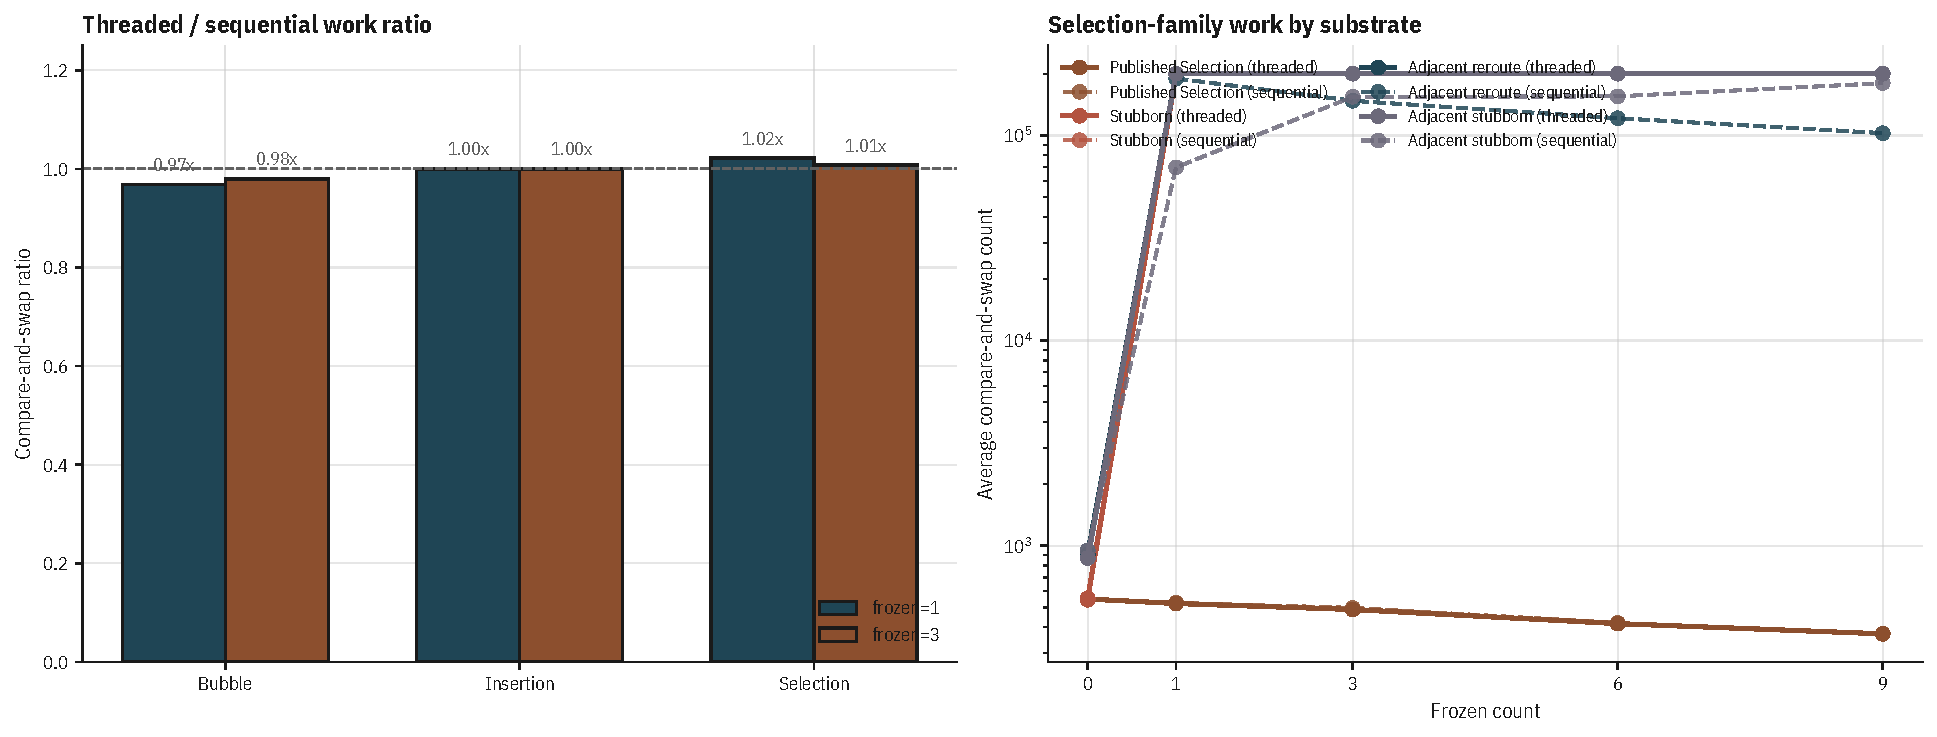
\includegraphics[width=\linewidth]{figures/fig8_substrate_work.pdf}
  \caption{\textbf{Threaded and sequential cell-view schedules do the same work.}
  Left: threaded/sequential compare-count ratios for the original trio under frozen counts $1$ and
  $3$. Right: Selection-family compare counts by substrate across frozen counts. Published
  Selection does the same work under either schedule, and the failing Selection variants run to
  the compare budget or the timeout under both.}
  \label{fig:exp26}
\end{figure}

\subsection{2D ordering boundary under shell targets}
The move from 1D to 2D is not merely a quantitative scaling but a qualitative change in the
structure of the problem. In 1D, any inversion can eventually be resolved by a sequence of adjacent
swaps: every pair of elements that need to exchange relative order will, at some point, become
neighbors. In 2D with a non-trivial target order such as shell distance, two values that must
exchange relative order may be separated by cells that cannot be permuted by local swaps
alone. This creates non-adjacent inversions that require multi-step routing through the grid, acting
as the 2D analogue of the combinatorial barrier that makes frozen cells fatal for Bubble in 1D,
except that in 2D the barrier exists even without frozen cells.

This section regenerates from a single canonical raw-trial archive (Appendix~\ref{sec:appendix-repro})
and derives the Figure~3 summaries from that source.
We still treat the 2D evidence as narrower than the 1D core because it covers a small
set of operator/target combinations, but its provenance is now explicit and reproducible.

Under the shell-based target order (value increases with squared distance from origin),
we observe a clear boundary:
Bubble2D fails to solve the task, while Selection2D succeeds in the obstacle-free case and then
collapses under immovable frozen cells, with only one small nonzero condition
($4\%$ success on the $6{\times}6$, 8-neighbor, 3-frozen condition).
Figure~\ref{fig:2d-heatmaps} summarizes success rates across grid sizes and neighborhood connectivities.

\paragraph{Alternative ordering targets.}
To confirm that this boundary is not an artifact of the shell-distance target, the canonical 2D
pipeline also evaluates row-major and serpentine (boustrophedon) ordering targets.
Under row-major ordering, the local algorithm (LocalOrder2D) achieves $0\%$ success even without
frozen cells, because row-major introduces non-adjacent inversions that purely local swaps cannot
resolve. Under serpentine ordering (which preserves locality along the space-filling path), the
local algorithm achieves $100\%$ at zero frozen cells but its performance collapses once frozen
cells are introduced, with only one small nonzero condition in the canonical archive
($6\%$ success on the $6{\times}6$, 8-neighbor, 3-frozen setting). SelectionOrder2D achieves
$100\%$ at zero frozen cells across all orderings and connectivities, but also collapses under
frozen cells, retaining only sparse nonzero success in a few $6{\times}6$ conditions.
These controls qualify rather than erase the shell-order boundary: target-order choice can rescue a
purely local algorithm in the zero-obstacle case (serpentine), but not under row-major ordering or
once frozen cells are introduced.

\begin{figure}[t]
  \centering
  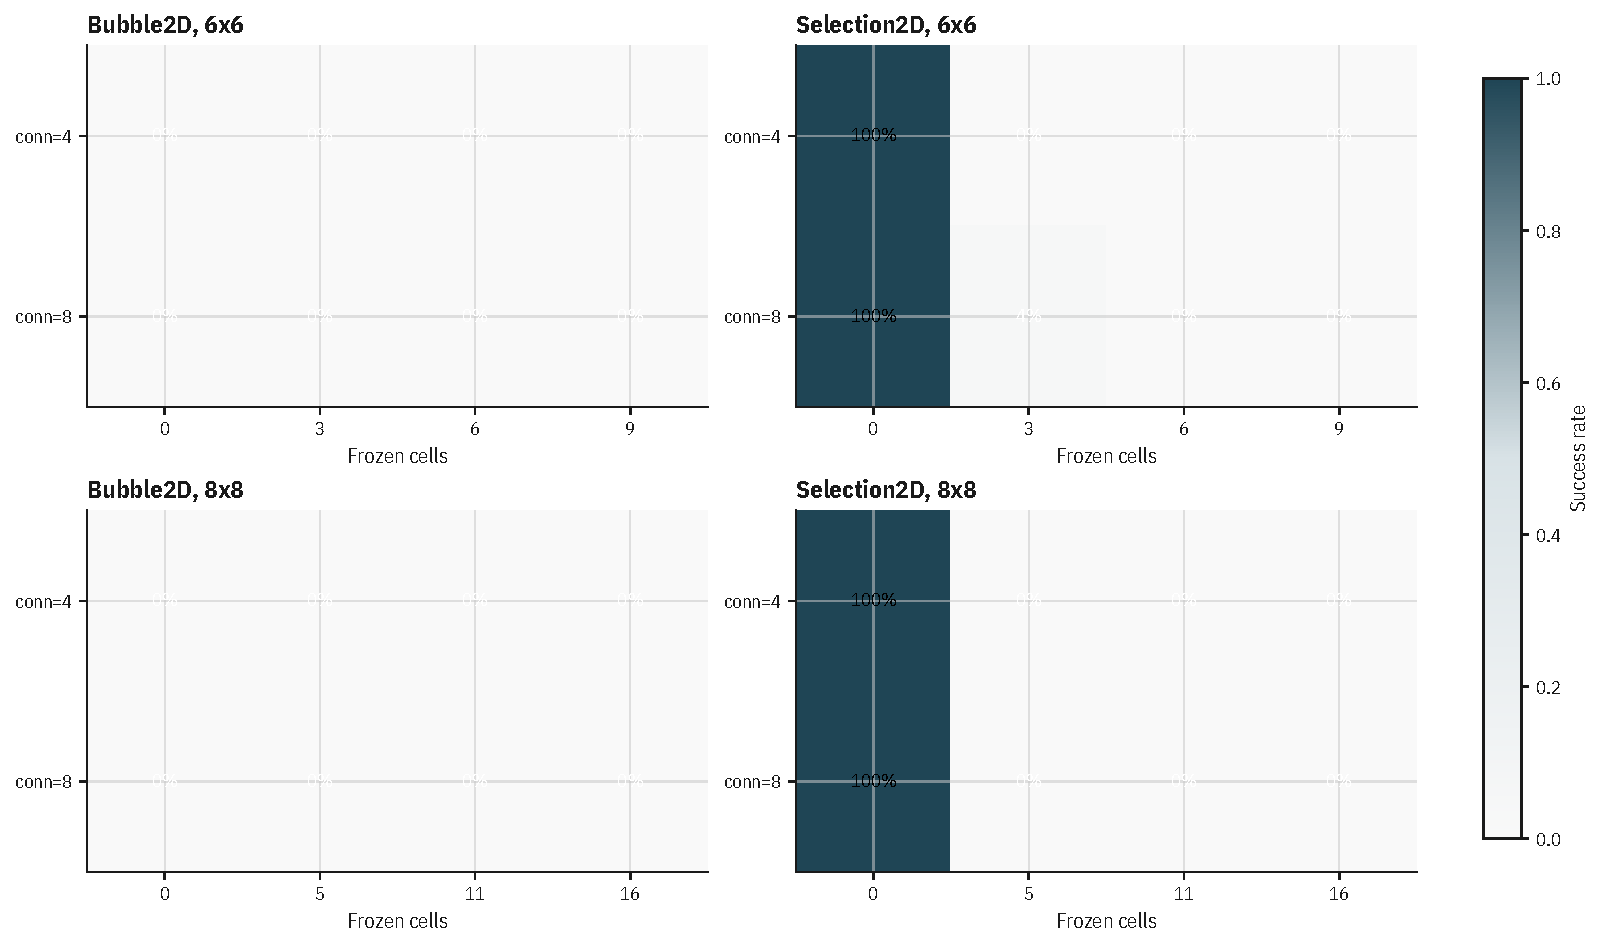
\includegraphics[width=\linewidth]{figures/fig3_2d_success_heatmaps.pdf}
  \caption{\textbf{Canonical 2D success heatmaps (shell ordering).}
  Success rates for Bubble2D and Selection2D across frozen counts and 4/8-connectivity, for grid
  sizes $6\times 6$ and $8\times 8$. Results summarize $100$ trials per configuration, with
  max-steps set to $30\cdot \text{grid\_size}^2$. Even when 8-connectivity expands the local
  neighborhood, purely local algorithms do not reliably escape 2D local minima under this target
  order.}
  \label{fig:2d-heatmaps}
\end{figure}

\subsection{Dip trajectories: delayed gratification}
The paper's ``delayed gratification'' claim is that cells may temporarily worsen a global error
metric to achieve later improvement. We quantify this across $50$ trials per condition.

In 1D with $n=30$ and 3 movable frozen cells, $100\%$ of Bubble runs exhibit at least one dip
(mean $34.8$ dips per trial, mean depth $0.9$ monotonicity errors, mean recovery $2.0$ steps),
while $98\%$ of Selection runs do (mean $3.7$ dips, mean depth $0.5$, mean recovery $0.7$ steps).
In 1D, Bubble is substantially more dip-prone: its local dynamics generate many small oscillations
around movable obstacles, whereas Selection's temporary regressions are rare, shallow, and quickly
resolved. On this metric, 1D dip statistics do not cleanly track goal-directedness; they mostly
capture local thrashing. We have not compared these counts with a random-walk null at matched swap
counts, nor tested the rise of dips with frozen count that Zhang et al.\ use to argue that the
dips are not a random walk, so the statistics describe the trajectories without testing that
argument. The script that produces them still starts threads for frozen cells, which adds
contention but no swaps, since a frozen cell never initiates one.

In 2D ($6{\times}6$ grid, 3 immovable frozen cells), $100\%$ of Selection2D runs exhibit dips
(mean $308.7$ per trial, mean depth $3.6$ shell inversions, mean recovery $7.2$ steps), while
Bubble2D shows no detected dips. Under this shell-order metric, Bubble2D stalls without producing
recoverable peaks, so the delayed-gratification signature becomes informative only in 2D, where the
goal-directed algorithm generates sustained progress against which temporary setbacks can be
measured.

Figure~\ref{fig:dips} shows representative trajectories; these are fixed-seed exemplars chosen as
the first dip-bearing trial when one exists, otherwise the first trial. They are not restricted to
successful runs and are not cherry-picked outliers.

\begin{figure}[t]
  \centering
  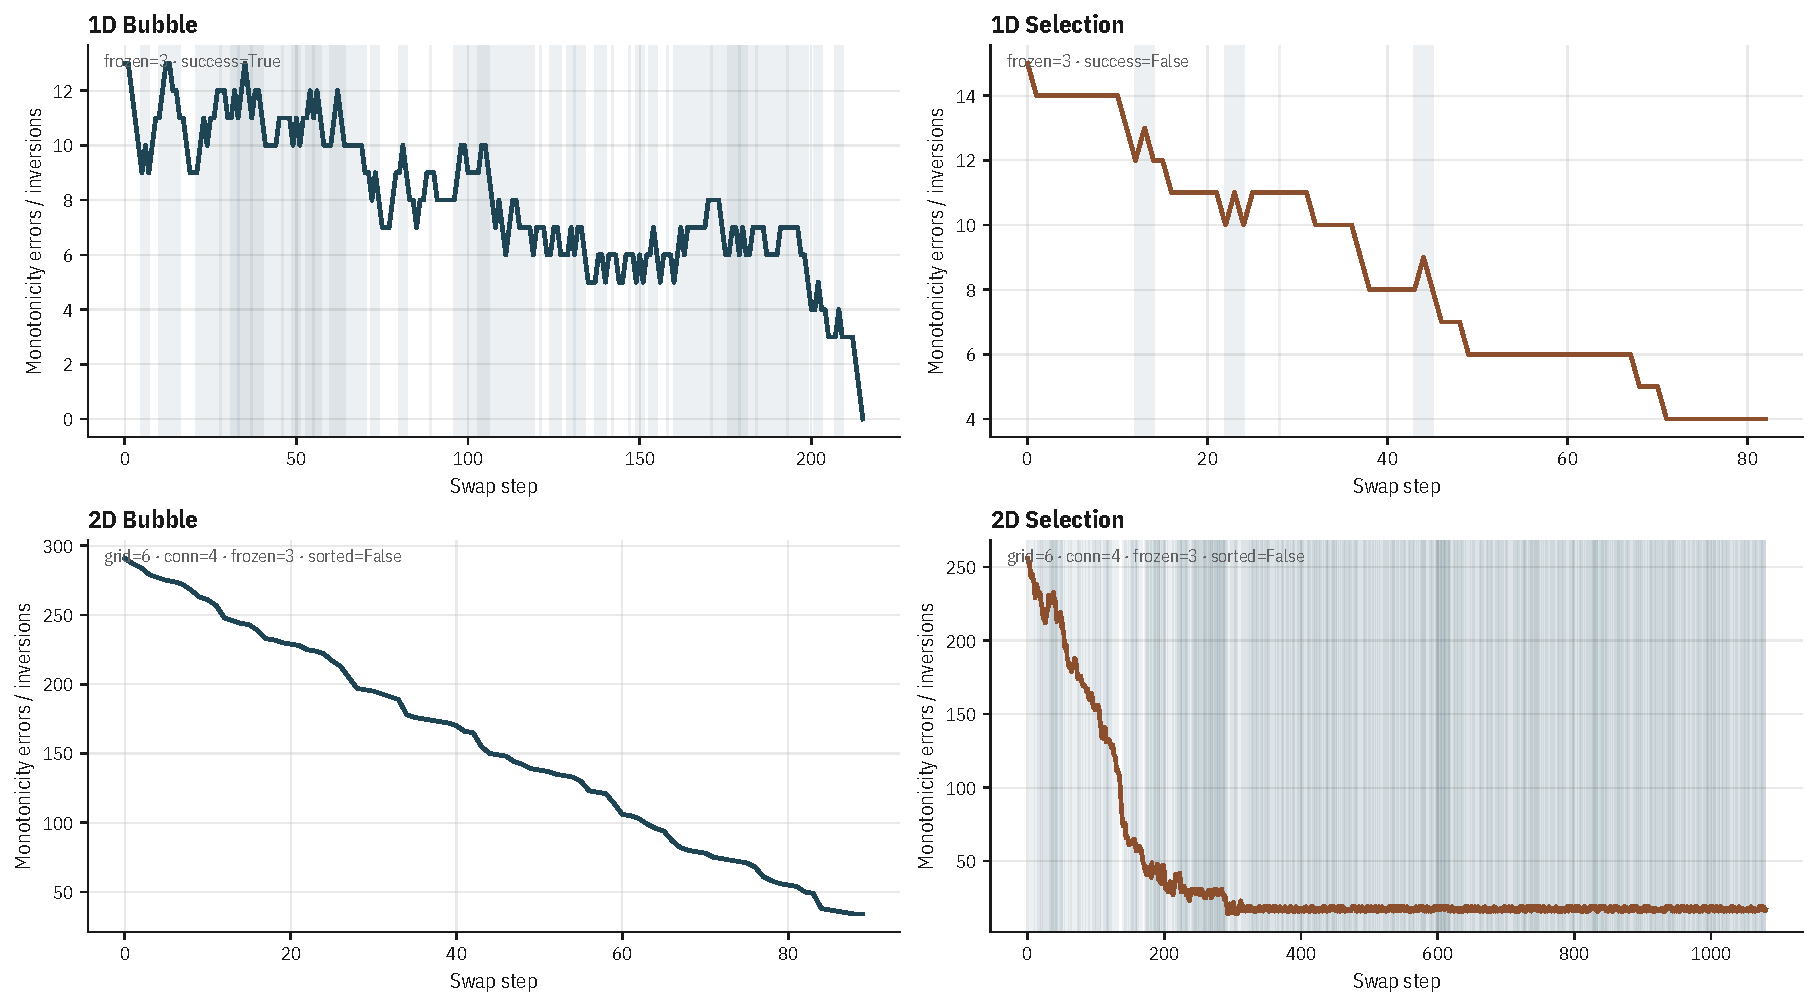
\includegraphics[width=\linewidth]{figures/fig4_dip_trajectories.pdf}
  \caption{\textbf{Dip trajectories (representative).}
  Shaded regions denote detected dip intervals where error temporarily increases and then recovers.
  Top row: 1D monotonicity errors under movable frozen cells. Bottom row: 2D inversion count under
  immovable frozen cells (shell ordering). Aggregate dip statistics across $50$ trials are reported
  in the text.}
  \label{fig:dips}
\end{figure}

\subsection{Topological signature and an algorithm-aligned progress diagnostic}
We apply persistent homology \cite{ghrist2008barcodes} to the swap-interaction graph: nodes are cells and edge weights are
swap frequencies; distances are set as $d = 1/(1+\text{swap\_count})$ and H1 features are computed
via \texttt{ripser} \cite{bauer2021ripser}. In 1D, H1 sharply differentiates Selection from local algorithms; in 2D, H1
counts remain high for both a failing algorithm (Bubble2D: mean $25.6$, success $0\%$) and a
successful one (Selection2D: mean $19.9$, success $100\%$).

This reveals that undirected H1 cycle count conflates local thrashing (Bubble) with directed
goal-seeking (Selection). As a descriptive follow-up, we compute a \emph{Directed Flow} metric: the
ratio of distance-reducing swaps (where the initiating cell moves closer to its ideal position) to
distance-increasing or neutral swaps. For Selection2D this metric is aligned with the same
ideal-position representation used by the policy itself, so we treat it as an algorithm-aligned
diagnostic rather than as independent evidence of competency. On the shell-order $6{\times}6$,
4-neighbor, no-frozen condition used in the right panel of Figure~\ref{fig:h1}, Bubble2D produces
$1835$ forward and $967$ backward initiator swaps across $30$ trials (ratio $1.90$), whereas
Selection2D produces $8741$ forward and $0$ backward initiator swaps. Even with that caveat, the
contrast is useful as a descriptive difference between local thrashing and policy-aligned progress.
Topological complexity alone is not evidence of problem-solving success.

\begin{figure}[t]
  \centering
  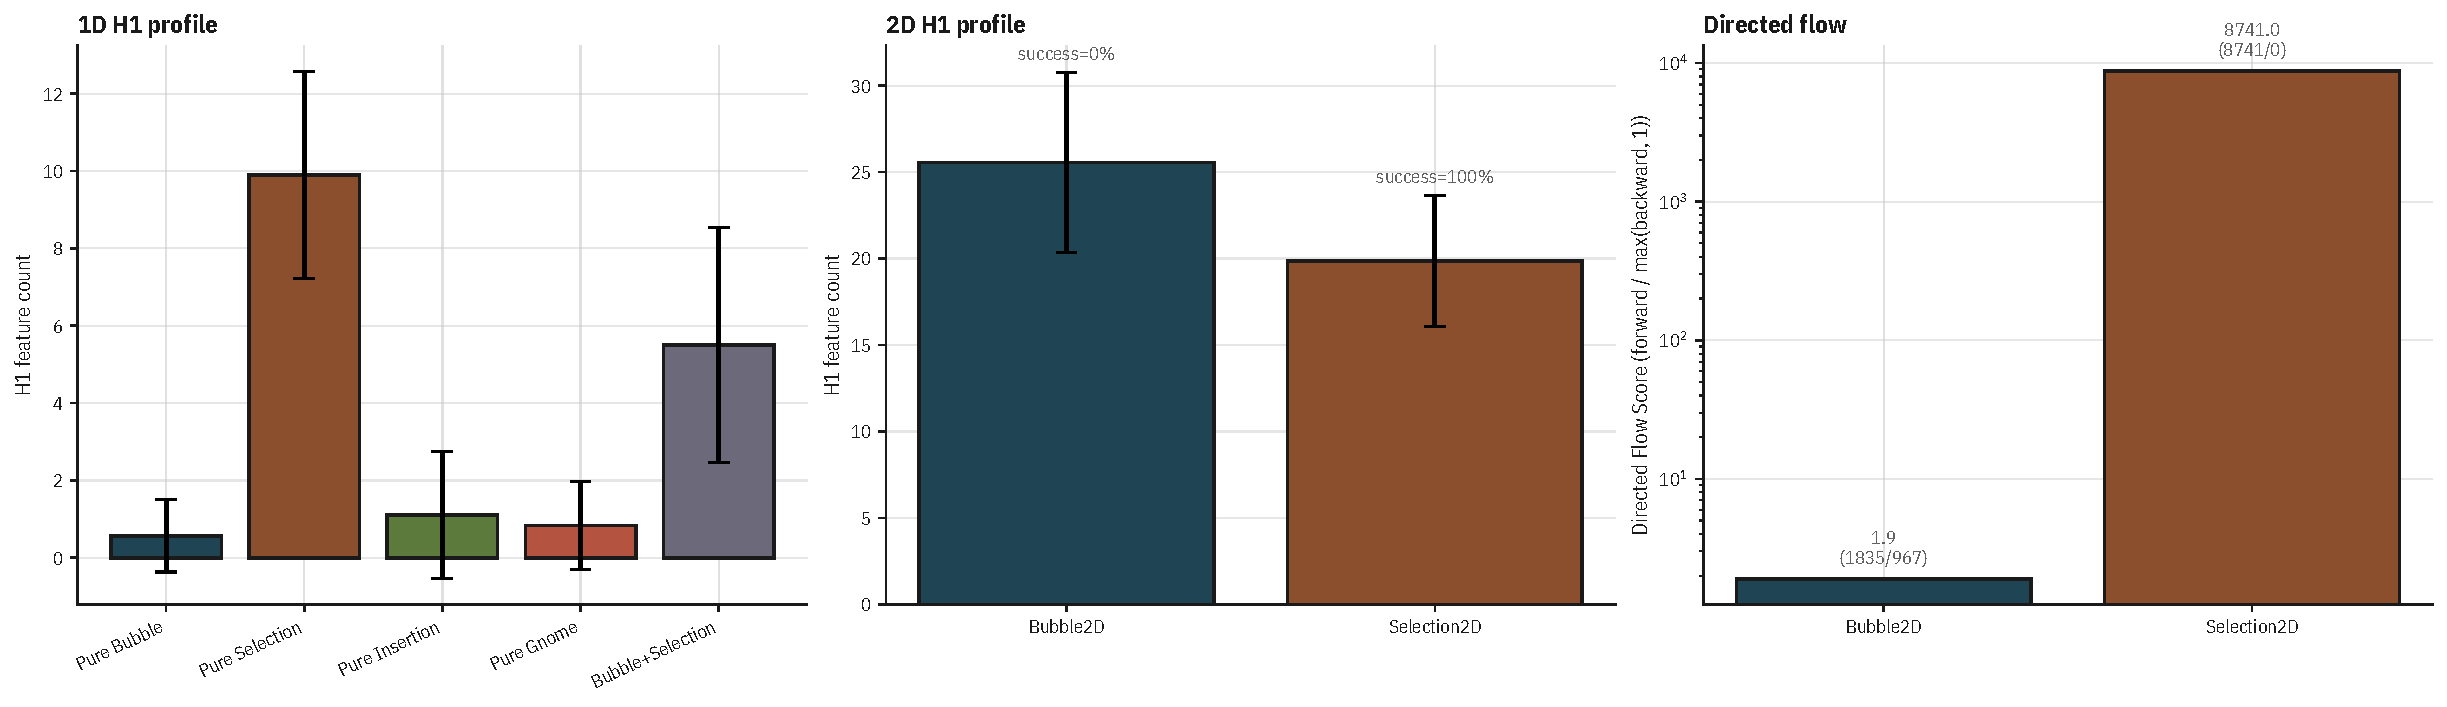
\includegraphics[width=\linewidth]{figures/fig5_h1_bar.pdf}
  \caption{\textbf{H1 features vs.\ Directed Flow.}
  Left/Middle: Undirected H1 separates 1D algorithms but fails to distinguish a failing algorithm (Bubble2D) from a successful one (Selection2D) in 2D. Right: Directed Flow is a useful descriptive diagnostic on the shell-order $6\times 6$, 4-neighbor, no-frozen condition, but because it is defined with respect to each cell's ideal position it should be read as policy-aligned rather than task-neutral. H1 statistics use $30$ trials; Directed Flow uses $30$ trials per 2D condition.}
  \label{fig:h1}
\end{figure}

\section{Matched State-Space Search Efficiency ($K_{\mathrm{state}}$)}
\label{sec:k-computation}
Chis-Ciure and Levin \cite{chisciure2025cognition} operationalize intelligence as search efficiency
in a problem space $\mathcal{P} = \langle S, O, C, E, H \rangle$, where $S$ is the state space,
$O$ the set of operators (with costs), $C$ the constraint set (forbidden state-operator pairs),
$E$ an evaluation functional, and $H$ the effective look-ahead horizon.
The K metric compresses the ratio of blind to guided search cost into a logarithmic scale:
\[
K \;=\; \log_{10}\!\left(\frac{\tau_{\text{blind}}}{\tau_{\text{agent}}}\right),
\]
where $\tau_{\text{blind}}$ is the expected cumulative cost under a maximal-entropy (unbiased)
random walk and $\tau_{\text{agent}}$ is the expected cost under the system's actual policy
\cite{fields2022competency}.
$K = 0$ marks chance; each integer increment corresponds to one order of magnitude of search
advantage.
Exact operator-walk K is therefore the reference target. Direct computation is intractable at
$n=30$, where the reachable spaces range up to $30!$ states, and blind random walks are too sparse
to give a practical first-hit estimate at the paper scale. We therefore report
$K_{\mathrm{state}}$: an exact reachable-state proposal null using the same operator family,
constraints, and cost function. $K_{\mathrm{state}}$ preserves the state-space scale and
matched-cost contract, but intentionally omits operator-graph traversal geometry.

\paragraph{Problem-space mapping.}
We therefore restrict the metric to the immovable
factorization, where operator classes and frozen-index constraints are explicit and fixed within
each condition. The sorting-cell model then instantiates the formalism as follows:
\begin{itemize}
  \item $S$: the reachable active-value permutations for a fixed frozen-index pattern.
  For long-range Selection, any permutation of the active values is reachable, so
  $|S| = (n_{\text{active}})!$. For adjacent sorting under immovable barriers, only within-segment
  permutations are reachable, so $|S| = \prod_r s_r!$ where $s_r$ are the active segment lengths.
  \item $O$: two matched operator families. The long-range family uses active-active transpositions;
  the adjacent family uses active-active adjacent swaps.
  \item $C$: immovable frozen indices remove state-operator pairs. For the adjacent family, this
  can disconnect the initial state from the goal entirely; for the long-range family, it reduces
  the active state space without eliminating transpositions across frozen barriers.
  \item $E$: active-subsequence sortedness, equivalent to zero inversion count after removing frozen
  indices from the readout.
  \item $H$: the finite factorization-trial horizon.
\end{itemize}

\paragraph{$K_{\mathrm{state}}$ results.}
Exact maximal-entropy operator-walk hitting times on these $n=30$ state graphs are intractable, so
we make the null explicit at the state-space level. Our blind baseline proposes a reachable state
uniformly at random and pays the matched mean operator cost per proposal, giving
\[
\tau_{\text{blind}}^{\text{state}} \;=\; |S_{\text{reachable}}| \,\bar{w},
\]
where $\bar{w}$ is the mean admissible operator cost under the relevant family and frozen pattern.
For the long-range family we use a distance-weighted transposition cost $w(o)=|i-j|$; for the
adjacent family this reduces to $w(o)=1$. Agent cost uses the realized span-weighted move cost per
attempt, $c = \texttt{total\_move\_distance}/2$, and folds failures into an effective cost-to-first-
success
\[
\tau_{\text{agent}}^{\text{eff}} \;=\; \bar{c}/p_{\text{success}},
\]
computed over reachable trial instances only. If $p_{\text{success}} = 0$, $K_{\mathrm{state}}$ is undefined.
This null is exact for the stated state-proposal process, not for a maximal-entropy operator walk.

Under this definition, all four Selection-family variants show large positive
$K_{\mathrm{state}}$ at frozen$=0$: published long-range Selection and its stubborn no-frozen control both achieve
$K_{\text{state}} \approx 30.45$ and $30.44$, while the adjacent variants achieve
$K_{\text{state}} \approx 29.81$ and $29.82$. Under immovable frozen indices, the matched long-range
rerouting curve declines monotonically as the reachable state space shrinks from $30!$ to $21!$:
$30.45 \rightarrow 26.14 \rightarrow 22.00 \rightarrow 18.01$ for frozen counts
$0,3,6,9$. These values sit $1.97$, $1.90$, $1.79$ and $1.70$ units below
$\log_{10}(n_{\text{active}}!)$ ($32.42$, $28.04$, $23.79$, $19.71$), and the adjacent values at
frozen$=0$ sit about $2.6$ units below it, so the size of the reachable state space sets almost all
of $K_{\mathrm{state}}$ and the agent's cost moves it by about two units. By contrast, long-range stubborn Selection has $K_{\text{state}}$ only at frozen$=0$; it
becomes undefined as soon as any frozen indices are introduced because success drops to $0/30$.

The adjacent family exposes a different K-based failure mode. At frozen$=0$, both adjacent variants
have well-defined positive $K_{\text{state}}$, but at frozen $3/6/9$ the adjacent-plus-immovable
problem space is disconnected for every sampled factorization trial: reachable fraction $0/30$ in each
condition. Thus $K_{\mathrm{state}}$ is undefined there for structural reasons, not merely because the policy is bad.
This is precisely the operator-and-constraint point the previous mixed K surface obscured.

\begin{figure}[t]
  \centering
  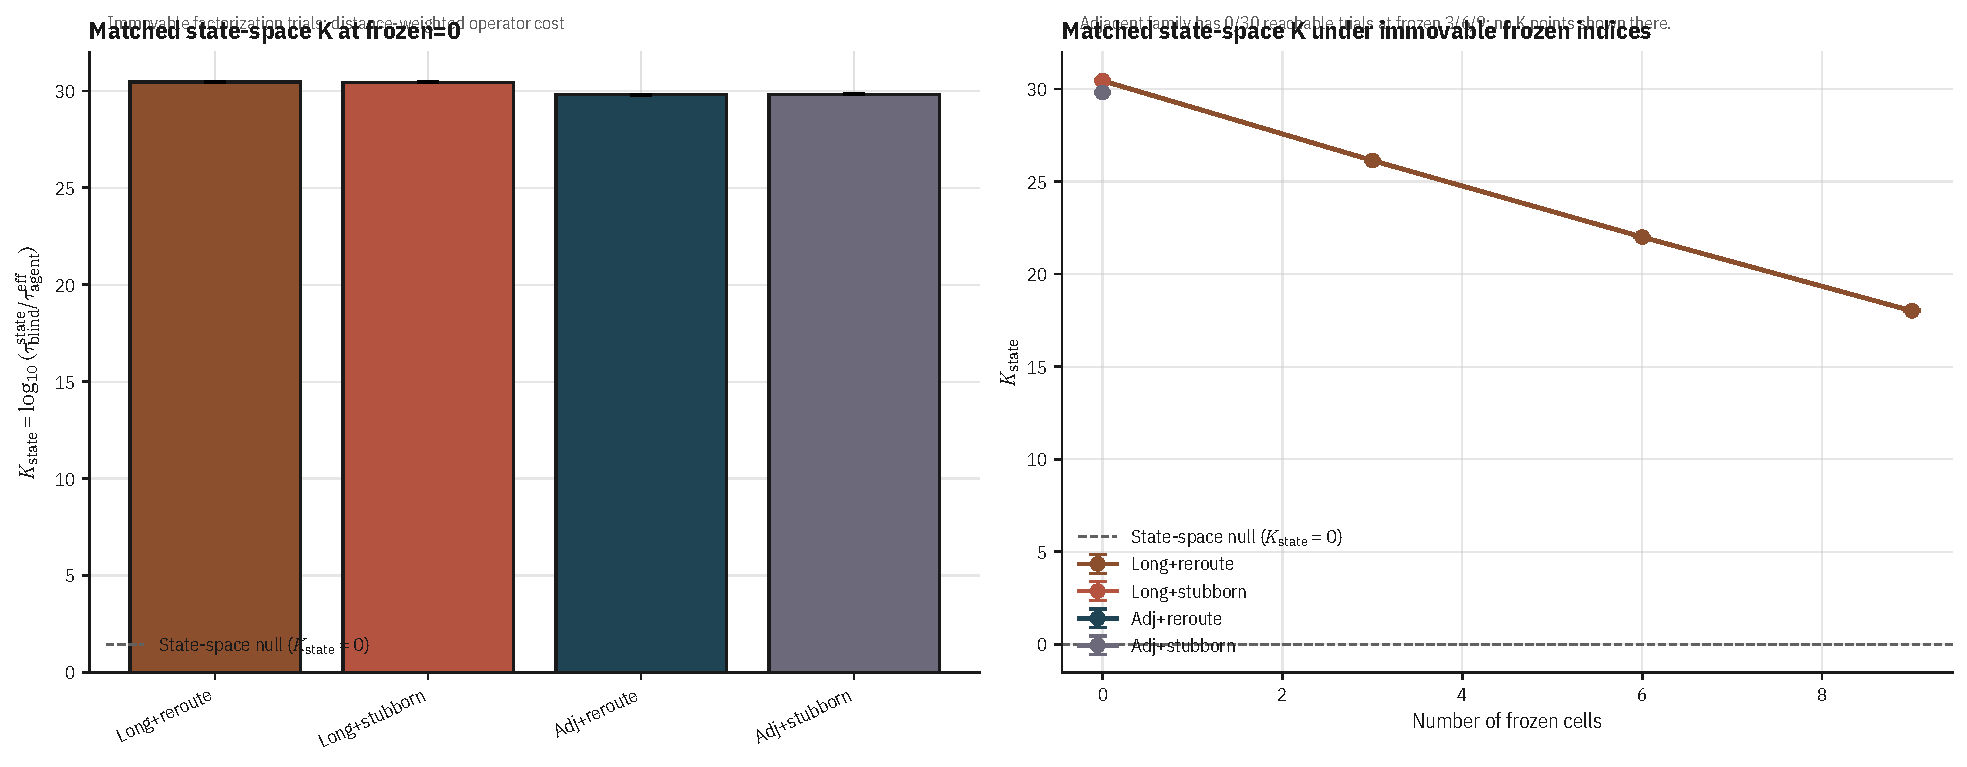
\includegraphics[width=\linewidth]{figures/fig6_k_values.pdf}
  \caption{\textbf{Matched state-space K on the immovable factorization.}
  Left: all four Selection-family variants have large positive exact $K_{\mathrm{state}}$ at frozen$=0$, but the
  adjacent variants are weaker because they spend more span-weighted work to traverse the same
  reachable state space. Right: when the exact state-space blind baseline is recomputed under each
  frozen pattern, long-range rerouting remains strongly supra-random while declining with the
  active state-space size. Long-range stubborn has undefined $K_{\mathrm{state}}$ once success drops to zero. The
  adjacent family has no reachable trial instances at frozen $3/6/9$, so no $K_{\mathrm{state}}$ points appear there.
  Error bars show 95\% bootstrap CIs.}
  \label{fig:k-values}
\end{figure}

\paragraph{Interpretation.}
This $K_{\mathrm{state}}$ surface is exact for an explicit state-space null tied to explicit
operator families, frozen constraints, and a distance-weighted cost model, and it should be read as
a scalable state-space proxy for the formal K target rather than as an operator-walk hitting-time
calculation. Because the null's size dominates it, the decline with frozen count and the
separation between a reachable-but-failing stubborn policy and an unreachable adjacent problem
restate the factorization, and any competency signal beyond reachability lives in the two units
that the agent's realized cost contributes.

\section{Discussion}
\label{sec:discussion}
\paragraph{Mechanism-first interpretation.}
Clustering in the gated mixtures does not require attraction, communication of type, or explicit
coordination. When one type is active early and the other late, swaps occur in temporally
correlated bursts that leave the currently active type adjacent to itself, which is the efficiency
hypothesis of Zhang et al.\ in mechanistic form. The reading has a developmental counterpart in
heterochrony, where shifts in the relative timing of developmental events generate morphological
diversity \cite{gould1977ontogeny}; here the ``developmental events'' are sorting phases, and a
timing shift between them produces spatial pattern without a patterning instruction. Removing the
gate returns clustering to the null, and transplanting it onto Bubble and Gnome clones raises
clustering to the level of native Insertion, so for these mixtures the timing shift is both
necessary and sufficient within the conditions we tested. Timing does not explain the weak
clustering of Selection mixtures, which arises at separations close to those of the ungated
controls, nor the aggregation that Zhang et al.\ report in the final state of their
duplicate-value runs, where a transient timing effect should have washed out; both point to a
second mechanism that we have not tested.

\paragraph{Active-matter framing (MIPS).}
The clustering mechanism has a MIPS-like mobility-separation analogy: algorithmic rules define
effective motility profiles, and Insertion remains quiescent until its enable-to-move condition is
met, so that the late-moving type rearranges among itself while the early type has settled. The
InsertionNoWait ablation equalizes the motility profiles and returns clustering to the null,
consistent with this interpretation.

\paragraph{Exclusion-process framing (inhomogeneous TASEP).}
The 1D lattice with hard-core exclusion suggests an exclusion-process analogy for the adjacent
immovable-barrier cases, in which frozen cells and high-latency algotypes act as transport defects.
These defects reduce local flux and induce jammed phases with upstream density buildup. Under
immovable constraints, local algorithms fail in ways consistent with persistent blockages, while
Selection’s non-local target assignment effectively bypasses local exclusion constraints.

\paragraph{Robustness is semantic and algorithmic.}
Robustness in this model depends on operator class, blocked-target policy, and obstacle semantics
(movable vs.\ immovable), and under immovable barriers most of the dependence is fixed by the rule
definitions. Adjacent active-active moves cannot exchange values across an immovable frozen index,
so the adjacent Selection variants, Bubble and Insertion all stop in a segment-sorted state; a
long-range Selection cell that keeps its frozen target waits forever; and only long-range Selection
with frozen-target rerouting can reach the sorted state. Cell-view and centralized implementations
that share the skip-frozen rule must then agree, and they do. The cell-view advantage in the
original comparison of cell-view and traditional algorithms most likely came from traditional
baselines without frozen-aware rerouting, so the competency worth studying is the rerouting rule
itself, Selection's frozen-target branch, rather than the cell-view framing.

The substrate comparison is narrower than it first appears. Every cell thread acquires one shared
lock before acting, so the threaded implementation is a serialized random scheduler with bursty
time slices, and once frozen cells run no thread it does the same work as a sequential random
schedule of the same cells. In this code there is no distributed substrate whose contribution could
be separated from the policy, and the agreement between substrates tells us that the
implementation behaves as its rules say rather than that competency is independent of substrate in
general. A physically embodied system without a global lock would be a separate test.

\paragraph{2D reveals limits of purely local information.}
The 2D shell-ordering target exposes non-adjacent inversions that local neighbor rules cannot resolve
reliably. Selection's explicit ideal position acts as a surrogate for positional information
\cite{wolpert1969positional}, suggesting a computational analogy: any system that must route
components to distant target positions through a constrained grid needs some form of non-local
information. Selection's ideal-position target is a minimal version of this, but it degrades under
frozen cells in 2D (unlike 1D), suggesting that two-dimensional morphogenesis demands richer
guidance signals than a static positional target alone. The section is now reproducible from a
canonical raw-trial archive, but it remains narrower in scope than the 1D factorization and
baseline results.

\paragraph{Search efficiency as a graded metric.}
The $K_{\mathrm{state}}$ analysis gives Chis-Ciure and Levin's formalism \cite{chisciure2025cognition}
a worked example with explicit $O$, $C$, and $w$, and the example shows how much of the value the
null carries. For every algorithm that finishes, $K_{\mathrm{state}}$ sits $1.7$ to $2.6$ units
below $\log_{10}(n_{\text{active}}!)$, so its decline with frozen count follows from the shrinking
reachable state space, and the two failure modes it separates (stubborn Selection keeps a reachable
space but never succeeds, the adjacent family loses reachability) restate the factorization. The
span-weighted agent cost enters only through those few units, which is where any
competency information beyond reachability would have to show. Because the blind numerator is
computed under a reachable-state proposal null rather than an exact maximal-entropy operator walk,
full operator-walk K remains for small-$n$ or separately bounded analyses, where the traversal
geometry that the proposal null omits would contribute.

\section{Related Work}
\label{sec:related}

\paragraph{The claims we test.}
Zhang et al.\ \cite{zhang2024classical} report that algotype clustering emerges in chimeric arrays
without explicit coordination and propose an efficiency hypothesis for it, in which efficient
algotypes move first and slower ones catch up; that cell-view versions of the algorithms reach
lower final error than traditional versions when some cells are frozen; and that the cells show
delayed gratification, a transient loss of sortedness that is recovered later, which rises with
the number of frozen cells. Their robustness comparison sets cell-view algorithms against
traditional algorithms, so it is a claim about the algorithms with their frozen-cell handling
rather than about distributed versus centralized execution. In the published implementation these
claims rest on specific operator semantics, since 1D Selection is not an adjacent-swap rule. We
test the clustering account by intervention, removing the waiting gate and transplanting it, and
we test the robustness comparison by giving the traditional baselines the same skip-frozen
rerouting and by changing only the execution schedule of the same cells. Their aggregation control
with identical algorithms reports values (0.57 to 0.65) well above the random-mixing baseline,
which the maximum-statistic bias described in Section~\ref{sec:methods} explains.

\paragraph{Morphogenesis and self-organization.}
Classic accounts of morphogenesis include reaction--diffusion pattern formation
\cite{turing1952chemical} and positional-information frameworks \cite{wolpert1969positional}.
Our temporal-separation result sits closer to the positional-information tradition: clustering
arises not from local chemical gradients but from timing differences between sorting phases,
analogous to heterochrony in developmental biology \cite{gould1977ontogeny}.

On the computational side, local-to-global coordination is central to distributed algorithms
\cite{lynch1996distributed}, swarm intelligence \cite{bonabeau1999swarm,couzin2009collective},
and swarm robotics \cite{rubenstein2014programmable,werfel2014designing}. The sorting-cell model is
distinguished by its extreme minimality: no explicit communication, no shared memory beyond the
array, and no coordination protocol.

\paragraph{Diverse Intelligence and K-computation.}
Levin's ``mind everywhere'' framework treats adaptive, goal-like behaviors as graded phenomena
across substrates \cite{levin2022technological}. Chis-Ciure and Levin \cite{chisciure2025cognition}
formalize this via the K-computation metric, operationalizing intelligence as search efficiency
in a problem space $\mathcal{P} = \langle S, O, C, E, H \rangle$. Our
$K_{\mathrm{state}}$ analysis provides a worked state-proposal approximation of how the abstract
formalism maps onto a specific model with explicit state spaces, operators, constraints, and costs.
Fields and Levin
\cite{fields2022competency} develop the broader theoretical context of competency navigation; we
ground their framework in a system small enough that every parameter is inspectable.

\section{Limitations}
\label{sec:limits}
\paragraph{Concurrency and nondeterminism.}
Bubble cells choose their swap direction at random, and the order in which threads acquire the
shared lock is set by the operating system, so fixing \texttt{random.seed} fixes the initial
arrays and frozen sets but does not make threaded runs reproducible; the original paper describes
the algorithms as deterministic, which holds for the textbook versions only. The reruns for this
revision ran several experiments concurrently on one machine, which changes thread timing and can
shift timeout-limited outcomes slightly. We report multi-seed aggregates and archive the compact
result files that feed every figure in \texttt{paper/results/}.

\paragraph{Frozen cells in the remaining scripts.}
The frozen-thread correction is applied in the factorization and matched-substrate experiments,
whose results we reran. The rerouting ablation, the centralized comparison and the dip statistics
still start threads for frozen cells. For the rerouting ablation and the centralized comparison
this affects work counts but not success, and their tables come from an earlier archive whose
per-seed files were not retained; the dip statistics were rerun with the same scripts.

\paragraph{Experiments of the original paper not followed up.}
We did not revisit the duplicate-value runs, in which Zhang et al.\ report that aggregation
persists into the final state, the opposite-direction chimeras and their incompletely sorted
equilibrium, the three-type mixture, the efficiency comparisons between algotypes, or the rise of
delayed gratification with frozen count. The duplicate-value result matters most for the timing
account, because clustering that survives to the final state cannot come from a transient timing
effect alone, and the frozen-count trend carries the original argument that the dips are not a
random walk, which our dip statistics do not test.

\paragraph{2D scope.}
The 2D archive now regenerates from a single canonical raw-trial pipeline, but the 2D evidence
still covers a narrower slice of the design space than the 1D core: two shell-order algorithms,
two alternate-order controls, and fixed step budgets. We therefore treat the 2D boundary as
reproducible but narrower in scope than the 1D factorization and substrate results. Directed Flow
and related progress diagnostics remain exploratory.

\paragraph{Semantics sensitivity.}
Several headline behaviors depend qualitatively on semantics that are easy to gloss over: whether
frozen elements are movable or immovable, how completion is detected, and which ordering target is
used in 2D. Claims about robustness or ``navigation'' should be interpreted only relative to an
explicitly stated semantics.

\section{Conclusion}
Scored against a label-permutation null on each run's own trajectory, algotype clustering in the
sorting-cell model appears where one class moves late. Removing Insertion's waiting gate returns
clustering to the null, and transplanting the same gate onto Bubble and Gnome clones reproduces the
clustering of native Insertion while the ungated clones stay at the null, which gives the
efficiency hypothesis of Zhang et al.\ a causal test it passes for gated mixtures. Selection
mixtures cluster weakly without temporal separation, and the original duplicate-value runs report
aggregation in the final state, so a second, non-timing mechanism remains open.

The robustness experiments come out the way the rule definitions require. Under immovable
obstacles only long-range Selection with frozen-target rerouting can reach the sorted state,
cell-view and centralized implementations that share the skip-frozen rule agree, and threaded and
sequential schedules of the same cells agree in outcome and work once frozen cells run no thread,
which removes the large work ratios of the earlier version. These results place the competency in
the rerouting rule and suggest that the original cell-view advantage came from baselines without
it. $K_{\mathrm{state}}$ is set mostly by the size of the reachable state space, and the 2D section
and Directed Flow remain narrower diagnostics.

The sorting-cell model remains useful because its components are inspectable, and once operator
set, obstacle semantics, baselines and nulls are stated explicitly it becomes a clean test bed for
separating mechanism from metaphor in the Diverse Intelligence program.

\appendix

\section{Experiment Semantics and Reproducibility}
\label{sec:appendix-repro}

\subsection{Per-experiment semantics and scale}
\begin{table}[h]
  \centering
  \footnotesize
  \setlength{\tabcolsep}{5pt}
  \renewcommand{\arraystretch}{1.08}
  \begin{tabularx}{\linewidth}{@{}p{0.30\linewidth} p{0.20\linewidth} p{0.14\linewidth} X@{}}
    \toprule
    Experiment surface & Obstacle semantics & Scale & Trials \\
    \midrule
    Pairwise clustering figures & Baseline (no frozen) & $n=30$ / $n=50$ & $50$ (pairwise summary), $20$ (ablation) \\
    Selection factorization & Immovable + movable control & $n=30$ & $10 \times$ 3 seeds (immovable), $5 \times$ 3 seeds (movable) \\
    Frozen-target rerouting ablation & Immovable & $n=30$ & $30 \times$ 3 seeds \\
    Centralized baseline comparison & Immovable & $n=30$ & $12 \times$ 3 seeds \\
    Matched substrate comparison & Immovable & $n=30$ & $3 \times$ 3 seeds (original trio), $3 \times$ 3 seeds (Selection family) \\
    Canonical 2D heatmaps & Immovable & $6{\times}6$, $8{\times}8$ & $100$ per configuration \\
    Dip exemplars & Movable (1D), immovable (2D) & $n=30$, $6{\times}6$ & Single exemplars; $50$ aggregate trials \\
    H1 / Directed Flow & Baseline (no frozen) & $n=30$, $6{\times}6$ & $30$ per condition \\
    Matched state-space K & Immovable & $n=30$ & Derived from factorization raw trials \\
    \bottomrule
  \end{tabularx}
  \caption{Per-experiment obstacle semantics, scale, and archive size. The repository keeps numeric script ids, but the main text refers to these surfaces descriptively.}
  \label{tab:semantics}
\end{table}

\subsection{Command index}
All experiments live in \texttt{dossiers/zhang-levin-playground/}. The repository keeps numeric
script ids for archival continuity; the main text refers to the same surfaces descriptively.

\paragraph{Clustering and timing.}
\begin{itemize}
  \item Pairwise temporal separation vs.\ clustering:
  \begin{quote}\small
  \texttt{\detokenize{uv run python paper/compute_fig1_temporal_clustering.py}}
  \end{quote}
  \item Clustering ablation:
  \begin{quote}\small
  \texttt{\detokenize{uv run python paper/run_clustering_ablation.py}}
  \end{quote}
  \item Synthetic timing-gate transfer:
  \begin{quote}\small
  \texttt{\detokenize{for s in 40 41 42; do}}\\
  \texttt{\detokenize{  uv run python exp27_timing_interventions.py}}\\
  \texttt{\detokenize{    --base-seed $s --n-trials 10}}\\
  \texttt{\detokenize{    --out paper/results/exp27_seed${s}_n50_t10.json;}}\\
  \texttt{\detokenize{done}}
  \end{quote}
  Aggregate with:
  \begin{quote}\small
  \texttt{\detokenize{uv run python paper/aggregate_exp27_timing_interventions.py --inputs ...}}
  \end{quote}
\end{itemize}

\paragraph{1D robustness and substrate comparisons.}
\begin{itemize}
  \item Selection factorization, immovable:
  \begin{quote}\small
  \texttt{\detokenize{for s in 40 41 42; do}}\\
  \texttt{\detokenize{  uv run python exp25_selection_factorization.py}}\\
  \texttt{\detokenize{    --seed $s --n-trials 10 --timeout 5 --semantics immovable}}\\
  \texttt{\detokenize{    --out paper/results/exp25_seed${s}_n30_t5_immovable.json;}}\\
  \texttt{\detokenize{done}}
  \end{quote}
  \item Selection factorization, movable control:
  \begin{quote}\small
  \texttt{\detokenize{for s in 40 41 42; do}}\\
  \texttt{\detokenize{  uv run python exp25_selection_factorization.py}}\\
  \texttt{\detokenize{    --seed $s --n-trials 5 --timeout 5 --semantics movable}}\\
  \texttt{\detokenize{    --out paper/results/exp25_seed${s}_n30_t5_movable.json;}}\\
  \texttt{\detokenize{done}}
  \end{quote}
  Aggregate with:
  \begin{quote}\small
  \texttt{\detokenize{uv run python paper/aggregate_exp25_selection_factorization.py --inputs ...}}
  \end{quote}
  \item Frozen-target rerouting ablation:
  \begin{quote}\small
  \texttt{\detokenize{for s in 40 41 42; do}}\\
  \texttt{\detokenize{  uv run python exp10_ablation_goal_adjustment.py}}\\
  \texttt{\detokenize{    --seed $s --n-trials 30 --timeout 10}}\\
  \texttt{\detokenize{    --out paper/results/exp10_seed${s}_n30_t10.json;}}\\
  \texttt{\detokenize{done}}
  \end{quote}
  \item Centralized baseline comparison:
  \begin{quote}\small
  \texttt{\detokenize{for s in 40 41 42; do}}\\
  \texttt{\detokenize{  uv run python exp14_cellview_vs_traditional.py}}\\
  \texttt{\detokenize{    --seed $s --n-trials 12 --timeout 10}}\\
  \texttt{\detokenize{    --out paper/results/exp14_seed${s}_n12_t10.json;}}\\
  \texttt{\detokenize{done}}
  \end{quote}
  \item Matched substrate comparison, original trio:
  \begin{quote}\small
  \texttt{\detokenize{for s in 40 41 42; do}}\\
  \texttt{\detokenize{  uv run python exp26_substrate_matched_baselines.py}}\\
  \texttt{\detokenize{    --seed $s --n-trials 3 --timeout 5}}\\
  \texttt{\detokenize{    --max-compare-and-swap 200000}}\\
  \texttt{\detokenize{    --frozen-counts 1,3 --algorithms Bubble,Insertion,Selection}}\\
  \texttt{\detokenize{    --out paper/results/}}\\
  \texttt{\detokenize{      exp26_original_trio_seed${s}_n30_t3_frozen1_3_budget200k.json;}}\\
  \texttt{\detokenize{done}}
  \end{quote}
  \item Matched substrate comparison, Selection family:
  \begin{quote}\small
  \texttt{\detokenize{for s in 40 41 42; do}}\\
  \texttt{\detokenize{  uv run python exp26_substrate_matched_baselines.py}}\\
  \texttt{\detokenize{    --seed $s --n-trials 3 --timeout 5}}\\
  \texttt{\detokenize{    --max-compare-and-swap 200000}}\\
  \texttt{\detokenize{    --frozen-counts 0,1,3,6,9}}\\
  \texttt{\detokenize{    --algorithms Selection,StubbornSelection,}}\\
  \texttt{\detokenize{      AdjacentSelection,AdjacentStubbornSelection}}\\
  \texttt{\detokenize{    --out paper/results/}}\\
  \texttt{\detokenize{      exp26_selection_family_seed${s}_n30_t3_budget200k.json;}}\\
  \texttt{\detokenize{done}}
  \end{quote}
  Aggregate either matched-substrate panel with:
  \begin{quote}\small
  \texttt{\detokenize{uv run python paper/aggregate_exp26_substrate_matched_baselines.py}}\\
  \texttt{\detokenize{  --inputs ...}}
  \end{quote}
\end{itemize}

\paragraph{2D, diagnostics, and figure generation.}
\begin{itemize}
  \item Canonical 2D archive and aggregation:
  \begin{quote}\small
  \texttt{\detokenize{uv run python exp28_2d_canonical.py}}\\
  \texttt{\detokenize{  --out paper/results/exp28_2d_canonical_trials.json}}\\
  \texttt{\detokenize{uv run python paper/aggregate_fig3_2d.py}}\\
  \texttt{\detokenize{  --input paper/results/exp28_2d_canonical_trials.json}}\\
  \texttt{\detokenize{  --heatmap-out paper/results/fig3_2d_success_heatmaps.json}}\\
  \texttt{\detokenize{  --alt-out paper/results/fig3b_alt_orderings.json}}
  \end{quote}
  \item Matched state-space K:
  \begin{quote}\small
  \texttt{\detokenize{uv run python paper/compute_k.py}}
  \end{quote}
  \item H1 summary:
  \begin{quote}\small
  \texttt{\detokenize{uv run python paper/compute_fig5_h1.py}}
  \end{quote}
  \item Directed Flow:
  \begin{quote}\small
  \texttt{\detokenize{uv run python paper/compute_directed_flow.py}}
  \end{quote}
  \item Dip statistics:
  \begin{quote}\small
  \texttt{\detokenize{uv run python paper/compute_dip_stats.py}}
  \end{quote}
  \item Figure generation:
  \begin{quote}\small
  \texttt{\detokenize{uv run python paper/make_figures.py}}
  \end{quote}
\end{itemize}

Thread scheduling introduces nondeterminism even with fixed RNG seeds. We therefore archive compact
JSON outputs (per-trial measurements and summaries, without state trajectories) in
\texttt{paper/results/} and report multi-seed aggregates. Every figure regenerates from those files.
The raw 2D trial archive (12.6\,MB) is regenerated by the seeded sequential 2D engine and kept out
of version control, with its Figure~3 aggregates tracked instead. The rerouting-ablation and
centralized-comparison tables (Table~\ref{tab:exp14} and the rerouting counts) come from an earlier
archive whose per-seed files were not retained, and both scripts still start threads for frozen
cells; rerunning them with the commands above regenerates comparable files.

\bibliographystyle{unsrt}
\bibliography{references}

\end{document}
